\section{Models}

\begin{table}[H]
	\centering
	\caption{Global rankings in 2014, 2015, 2016, 2017 Change in total headcount usage in the top 23 languages}
	\begin{tabular}{llrrrr}
		\toprule
		\multicolumn{1}{l}{Number} & Language & 2014  & 2015  & 2016  & 2017 \\
		\midrule
		1     & Chinese,Mandarin & 1052.535 & 1070.966 & 1073.525 & 1076.734 \\
		2     & Spanish & 441.7462 & 453.7809 & 466.8536 & 480.4602 \\
		3     & English & 816.9127 & 903.37 & 911.6737 & 917.9667 \\
		4     & Hindi & 365.4672 & 365.735 & 366.4932 & 367.5688 \\
		5     & Portuguese & 196.7223 & 198.126 & 200.7203 & 202.5036 \\
		6     & Bengali & 184.1833 & 186.2771 & 183.2275 & 179.4995 \\
		7     & Russian & 189.6124 & 192.1039 & 194.2471 & 197.3681 \\
		8     & Japanese & 124.9867 & 125.1537 & 125.3209 & 125.5303 \\
		9     & Javanese & 77.36284 & 76.93927 & 76.51803 & 75.99483 \\
		10    & German,Standard & 146.0954 & 146.6092 & 147.6057 & 148.2428 \\
		11    & Chinese,Wu & 73.22911 & 72.48929 & 71.75694 & 70.85228 \\
		12    & Korean & 117.8224 & 117.8665 & 117.9106 & 117.9658 \\
		13    & French & 126.9646 & 153.8068 & 154.9492 & 155.939 \\
		14    & Telugu & 81.37525 & 81.70919 & 82.14315 & 82.18562 \\
		15    & Marathi & 71.41339 & 71.47918 & 71.54502 & 71.62742 \\
		16    & Turkish & 58.45415 & 58.32959 & 58.2053 & 58.05032 \\
		17    & Tamil & 73.58453 & 73.5565 & 73.52849 & 73.4935 \\
		18    & Vietnamese & 67.34071 & 67.26303 & 67.18545 & 67.0886 \\
		19    & Urdu  & 153.8177 & 153.5716 & 153.3494 & 153.0674 \\
		20    & Italian & 64.94941 & 64.9459 & 64.94238 & 64.93799 \\
		\bottomrule
	\end{tabular}%
	\label{tab:addlabel}%
\end{table}%

\begin{figure}[H]
	\centering
	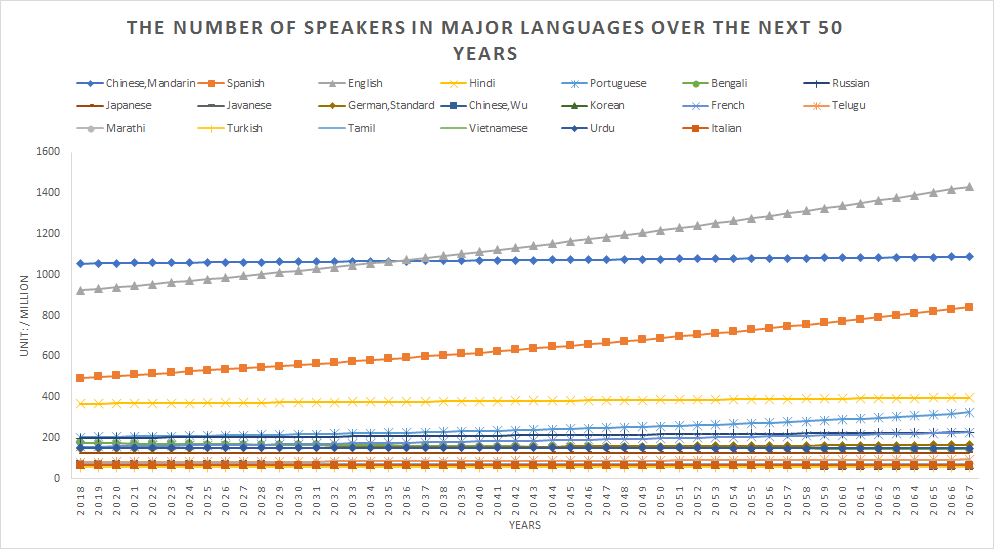
\includegraphics[width=1\linewidth]{figures/next50number}
	\caption{The number of speakers in major languages over the next 50 years}
	\label{fig:next50number}
\end{figure}

\begin{figure}[h]
	\centering
	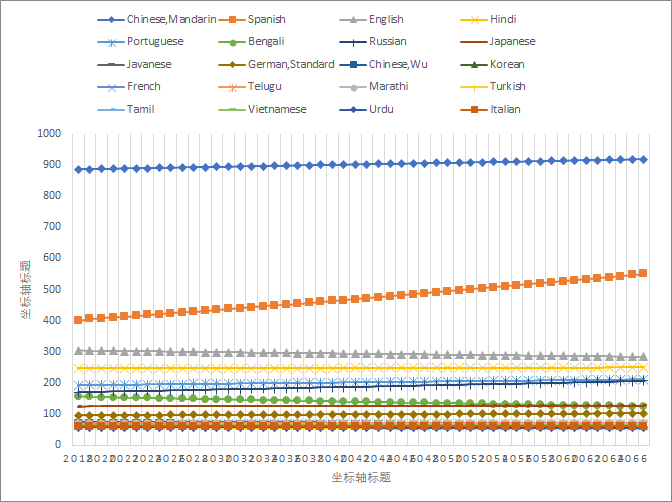
\includegraphics[width=1\linewidth]{figures/percent}
	\caption{}
	\label{fig:percent}
\end{figure}


\begin{figure}[H]
	\centering
	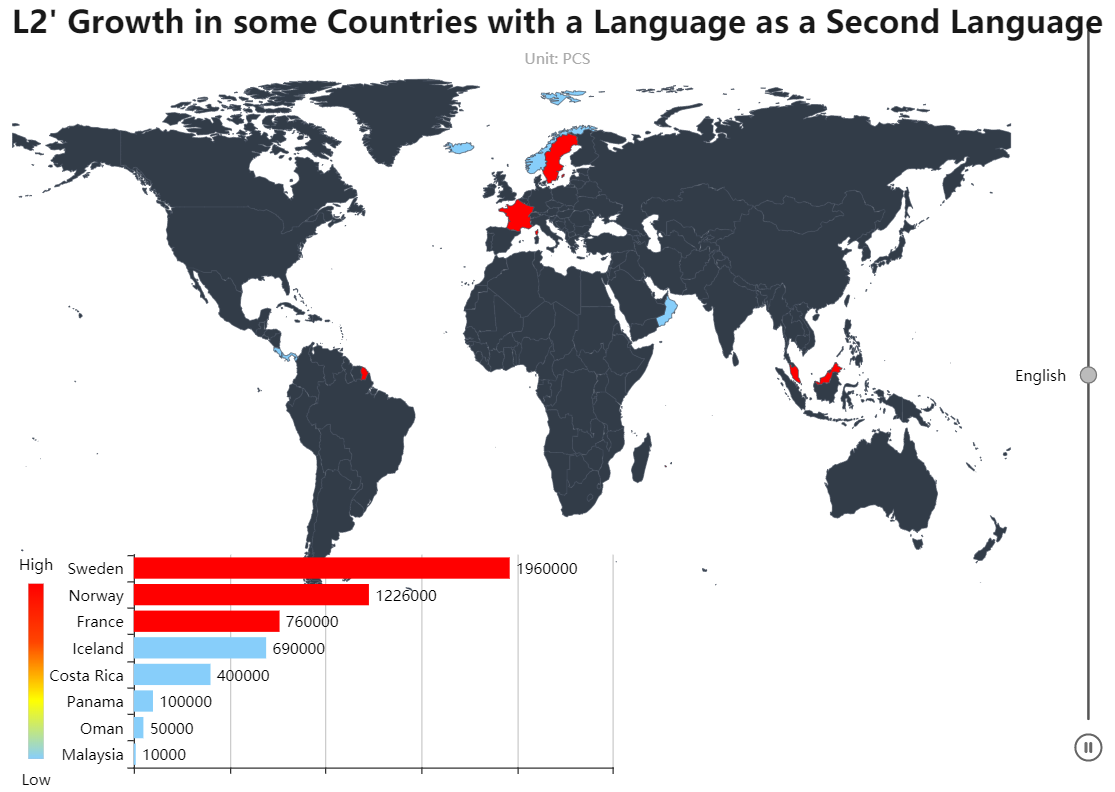
\includegraphics[width=1\linewidth]{figures/english}
	\caption{}
	\label{fig:english}
\end{figure}


\begin{figure}[h]
	\centering
	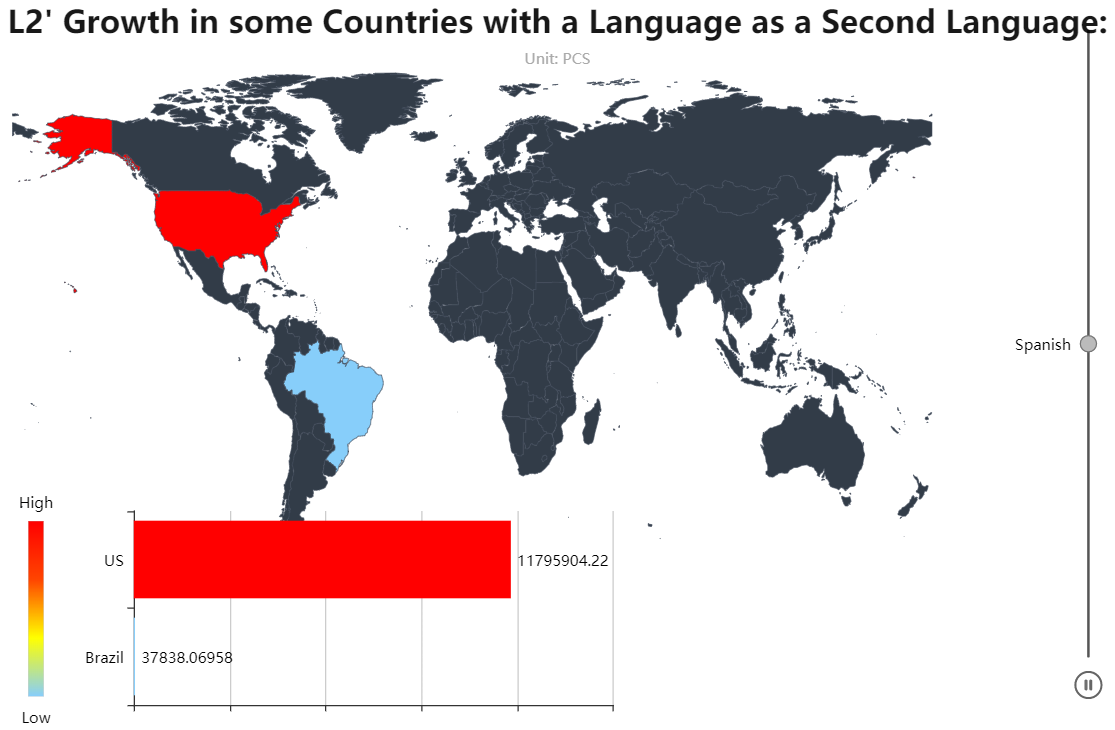
\includegraphics[width=1\linewidth]{figures/Spanish}
	\caption{}
	\label{fig:spanish}
\end{figure}



\begin{figure}
	\centering
	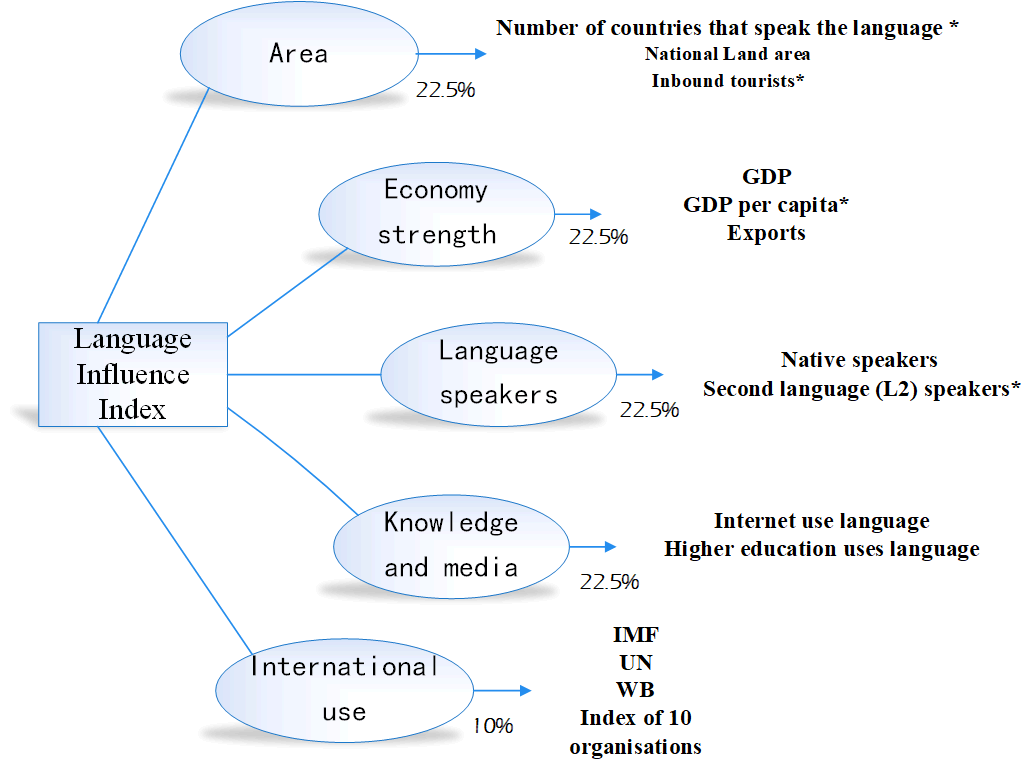
\includegraphics[width=1\linewidth]{figures/chart}
	\caption{Language Influence Index Structure chart}
	\label{fig:chart}
\end{figure}

% Table generated by Excel2LaTeX from sheet 'Sheet1'
\begin{table}[H]
	\centering
	\caption{Language ranking comparison}
	\begin{tabular}{l p{2.8cm}p{2.8cm}p{2.8cm}p{2.8cm}}
		\toprule
		\multicolumn{1}{l}{Rank} & native speakers(2017 year) & native speakers(2067 year) & total speakers(2017 year) & total speakers(2067 year) \\
		\midrule
		1     & Mandarin & Mandarin & Mandarin & English \\
		2     & Spanish & Spanish & English & Mandarin \\
		3     & English & English & Hindustani & Spanish \\
		4     & Hindustani & Hindustani & Spanish & Hindustani \\
		5     & Arabic & Portuguese & Arabic & Arabic \\
		6     & Bengali & Arabic & Malay & Portuguese \\
		7     & Portuguese & Bengali & Russian & Russian \\
		8     & Russian & Russian, & Bengali & French, \\
		9     & Punjabi & Japanese & Portuguese & German,Standard \\
		10    & Japanese & German Standard. & French & Malay \\
		\bottomrule
	\end{tabular}%
	\label{tab:addlabel}%
\end{table}%


% Table generated by Excel2LaTeX from sheet 'Sheet2'
\begin{table}[H]
	\centering
	\caption{ The second language is mainly used in countries / regions}
	\begin{tabular}{l|l|p{4cm} |p{4cm}}
		\toprule
		language & Asian & Europe & Oceania \\
		\midrule
		Chinese &       &       & Australian \\
			\midrule
		English &       & Sweden, France, Iceland, Poland &  \\	\midrule
		spanish &       &       &  \\	\midrule
		Arabic &       &       &  \\	\midrule
		Russian &       &Ukraine, Kazakhstan, Uzbekistan,Turkmen&  \\	\midrule
		Bengalese & India&       &  \\	\midrule
		Portuguese &       &       &  \\	\midrule
		French &       &       &  \\	\midrule
		Hausa &       &       &  \\	\midrule
		Turkish &       & Austria,Germany, Bulgaria &  \\	\midrule
		Italian &       &       &  \\
		\bottomrule
		\toprule
		language & North America& South America &  Africa \\
		\midrule
		Chinese &       &       &  \\	\midrule
		English & Central America & & Egypt,Sudan ,Cameroon ,Cameroon \\	\midrule
		spanish & \multicolumn{1}{l}{America} & Brazil &  \\	\midrule
		Arabic &       &       & Ethiopia ,Chad ,Somalia, South Sudan \\	\midrule
		Russian &       &       &  \\	\midrule
		Bengalese &       &       &  \\	\midrule
		Portuguese &       &       &  \\	\midrule
		French & America&       & Mozambique \\	\midrule
		Hausa &       &       & the Nile ,Nigeria \\	\midrule
		Turkish &       &       &  \\	\midrule
		Italian &       & Argentina & Algeria \\	\midrule
		\bottomrule
	\end{tabular}%
	\label{tab:addlabel}%
\end{table}%


% Table generated by Excel2LaTeX from sheet 'Sheet2'
\begin{table}[H]
	\centering
	\caption{012-2013 scores of some languages and rankings}
	 \scalebox{0.87}[0.87]{%
	\begin{tabular}{|p{4.11em}|r|r|r|r|r|r|}
		\toprule
		\multicolumn{1}{|c|}{\multirow{2}[4]{*}{\backslashbox[0pt][l]{Language}{Time}}} & \multicolumn{2}{c}{2012} & \multicolumn{2}{c}{2013} & \multicolumn{2}{c|}{2014} \\
		\cmidrule{2-7}    \multicolumn{1}{|c|}{} & \multicolumn{1}{p{4.11em}|}{Score} & \multicolumn{1}{p{4.11em}|}{Rank} & \multicolumn{1}{p{4.055em}|}{Score} & \multicolumn{1}{p{4.055em}|}{Rank} & \multicolumn{1}{p{4.055em}|}{Score} & \multicolumn{1}{p{4.055em}|}{Rank} \\
    \midrule
	English & 0.853  & 1     & 0.853  & 1     & 0.752  & 1 \\
	\midrule
	Chinese & 0.416  & 2     & 0.401  & 2     & 0.318  & 2 \\
	\midrule
	French & 0.301  & 5     & 0.302  & 4     & 0.200  & 7 \\
	\midrule
	Spanish & 0.398  & 3     & 0.401  & 3     & 0.307  & 3 \\
	\midrule
	Arabic & 0.278  & 7     & 0.275  & 7     & 0.202  & 6 \\
	\midrule
	Russian & 0.226  & 8     & 0.224  & 8     & 0.140  & 9 \\
	\midrule
	German & 0.280  & 6     & 0.276  & 6     & 0.268  & 5 \\
	\midrule
	Japanese & 0.179  & 9     & 0.180  & 9     & 0.153  & 8 \\
	\midrule
	Portuguese & 0.145  & 10    & 0.142  & 10    & 0.137  & 10 \\
	\midrule
	Hindi & 0.305  & 4     & 0.301  & 5     & 0.301  & 4 \\
	\bottomrule
	\end{tabular}%
}
	\label{tab:012}%
\end{table}%



% Table generated by Excel2LaTeX from sheet 'Sheet2'
\begin{table}[H]
	\centering
	\caption{Change of language performance rankings every decade}
	\begin{tabular}{|p{5.22em}|r|r|r|r|r|r|}
		\toprule
		\multicolumn{1}{|r|}{\backslashbox[0pt][l]{Language}{Year}} & 2017  & 2027  & 2037  & 2047  & 2057  & 2067 \\
		\midrule
		English & 1     & 1     & 1     & 1     & 1     & 1 \\
		\midrule
		Chinese & 2     & 2     & 2     & 2     & 2     & 2 \\
		\midrule
		French & 3     & 3     & 4     & 4     & 4     & 4 \\
		\midrule
		Spanish & 4     & 4     & 3     & 3     & 3     & 3 \\
		\midrule
		Arabic & 5     & 5     & 5     & 5     & 6     & 6 \\
		\midrule
		Russian & 6     & 6     & 6     & 6     & 5     & 5 \\
		\midrule
		German & 7     & 7     & 7     & 7     & 7     & 8 \\
		\midrule
		Japanese & 8     & 9     & 9     & 10    & 10    & 10 \\
		\midrule
		Portuguese & 9     & 8     & 8     & 8     & 9     & 9 \\
		\midrule
		Hindi & 10    & 10    & 10    & 9     & 8     & 7 \\
		\bottomrule
	\end{tabular}%
	\label{tab:Change}%
\end{table}%


